%%%%%%%%%%%%%%%%%%%%%%%%%%%%%%%%%%%%

\section{幾何分布}

%%%%%%%%%%%%%%%%%%%%%%%%%%%%%%%%%%%%

\subsection{ベルヌーイ分布}

%%%%%%%%%%%%%%%%%%%%%%%%%%%%%%%%%%%%

\begin{frame}
\frametitle{ミルグラム実験}

\twocol{0.6}{0.4}{

\begin{itemize}

\item イェール大学の心理学者スタンレー・ミルグラムは、1963年から権威への服従に関する一連の実験を行った。

\item 実験者（E）は教師（T）（実験の被験者）に対し、学習者（L）が質問に誤答するたびに強烈な電気ショックを与えるよう命令する。

\item 学習者は実際には俳優であり、電気ショックは本物ではないが、教師がショックを与えるたびに事前録音された音が再生される。

\end{itemize}

}
{
\begin{center}
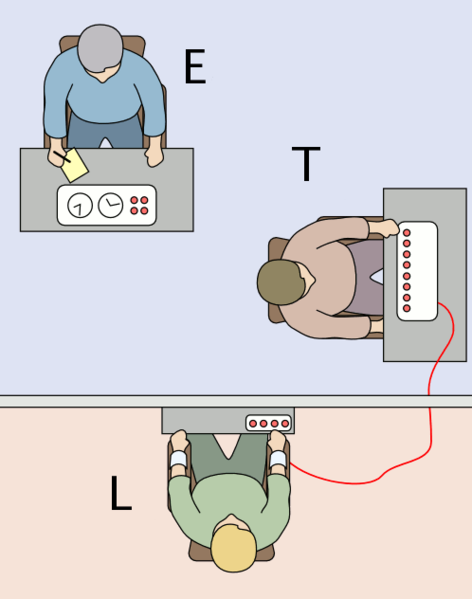
\includegraphics[width=\textwidth]{4-2_geometric_distribution/figures/milgram}
\end{center}
\ct{\webURL{http://en.wikipedia.org/wiki/File:Milgram_Experiment_v2.png}}
}

\end{frame}

%%%%%%%%%%%%%%%%%%%%%%%%%%%%%%%%%%%%

\begin{frame}
\frametitle{ミルグラム実験（続き）}

\begin{itemize}

\item これらの実験は、個人の良心に反する行為を指示する権威者に対して、研究参加者がどれほど従うかを測定した。

\item ミルグラムは、約65\%の人が権威に従い、そのようなショックを与えることを発見した。

\item 長年にわたる研究により、この数字はコミュニティや時代を超えてほぼ一定であることが示唆されている。

\end{itemize}

\end{frame}


%%%%%%%%%%%%%%%%%%%%%%%%%%%%%%%%%%%%

\begin{frame}
\frametitle{ベルヌーイ確率変数}

\begin{itemize}

\item ミルグラムの実験における各人は\hl{試行}と見なすことができる。

\item 強烈なショックを与えることを拒否した場合は\hl{成功}、ショックを与えた場合は\hl{失敗}とラベルを付ける。

\item ショックを与えることを拒否した人はわずか35\%であるため、\hl{成功確率}は \mathhl{p = 0.35} である。

\item 個々の試行に2つの結果しかない場合、それを\hl{ベルヌーイ確率変数}という。

\end{itemize}

\end{frame}

%%%%%%%%%%%%%%%%%%%%%%%%%%%%%%%%%%%%

\subsection{幾何分布}

\begin{frame}[shrink=15]
\frametitle{幾何分布}

{\small

\dq{スミス博士はミルグラムの実験を繰り返したいが、強烈なショックを与えない人が見つかるまでサンプリングしたいと考えている。最初の人でやめる確率は何か？}

\[ P(1\text{人目が拒否}) = 0.35 \]

\dq{……3人目の人でやめる確率は？}
\begin{align*}
P(\text{1人目と2人目がショック、3人目が拒否}) &= \slot{S}{0.65} \times \slot{S}{0.65} \times \slot{R}{0.35} \\
&= 0.65^2 \times 0.35 \approx 0.15
\end{align*}

\dq{……10人目の人でやめる確率は？}
\soln{
\begin{align*}
P(\text{9人がショック、10人目が拒否}) &= \underbrace{\slot{S}{0.65} \times \cdots \times \slot{S}{0.65}}_{9\text{個}} \times \slot{R}{0.35} \\
&= 0.65^9 \times 0.35 \approx 0.0072
\end{align*}
}
}

\end{frame}

%%%%%%%%%%%%%%%%%%%%%%%%%%%%%%%%%%%%

\begin{frame}
\frametitle{幾何分布（続き）}

\hl{幾何分布}は、\hl{独立同一分布（iid）}のベルヌーイ確率変数において、最初の成功までの待ち時間を記述する。
\begin{itemize}
\item 独立性：各試行の結果は互いに影響しない
\item 同一性：成功確率は各試行で同じ
\end{itemize}

$\:$ \\
$\:$ \\

\formula{幾何確率}{成功確率を $p$、失敗確率を $(1-p)$、独立試行回数を $n$ とすると \[P(n\text{回目の試行で初めて成功}) = (1-p)^{n-1} p\]}

\end{frame}

%%%%%%%%%%%%%%%%%%%%%%%%%%%%%%%%%%%%

\begin{frame}

\pq{サイコロを6回振って初めて6の目が出る確率を幾何分布で計算できるか？成功（6の目が出る）と失敗（6の目が出ない）は明確に定義されており、各試行でどちらかが必ず起こることに注意せよ。}

\begin{enumerate}[(a)]
\item いいえ、サイコロを振ると2つ以上の結果がある
\solnMult{はい、計算できる}
\end{enumerate}

\soln{
\[P(\text{6回目で初めて6の目}) = \pr{ \frac{5}{6} }^5 \pr{ \frac{1}{6} } \approx 0.067 \]
}

\end{frame}

%%%%%%%%%%%%%%%%%%%%%%%%%%%%%%%%%%%%

\begin{frame}
\frametitle{期待値}

\dq{スミス博士は、ショックを与えることを拒否する最初の人を見つけるまで、何人の人を試験すると予想されるか？}

幾何分布の期待値、すなわち平均は $\frac{1}{p}$ と定義される。
\[ \mu = \frac{1}{p} = \frac{1}{0.35} = 2.86 \]

スミス博士は、ショックを与えることを拒否する最初の人を見つけるまで、2.86人の人を試験すると予想される。

しかし、整数でない人数をどのように試験するのか？

\end{frame}

%%%%%%%%%%%%%%%%%%%%%%%%%%%%%%%%%%%%

\begin{frame}
\frametitle{期待値とその変動性}

\formula{幾何分布の平均と標準偏差}{
\[ \mu = \frac{1}{p} \qquad \qquad \sigma = \sqrt{\frac{1-p}{p^2}} \]
}

\begin{itemize}

\item スミス博士の実験に戻ると：

\[ \sigma = \sqrt{\frac{1-p}{p^2}} = \sqrt{\frac{1-0.35}{0.35^2}} = 2.3 \]

\item スミス博士は、ショックを与えることを拒否する最初の人を見つけるまで、平均2.86人（誤差±2.3人）の人を試験すると予想される。

\item これらの値は、実験を非常に多くの回数繰り返す文脈でのみ意味をなす。

\end{itemize}

\end{frame}

%%%%%%%%%%%%%%%%%%%%%%%%%%%%%%%%%%%%
